
\documentclass[11pt, letterpaper]{article}
%\usepackage{bookmark}
\usepackage[a4paper,margin=2cm]{geometry}
\usepackage[]{graphicx}
\usepackage{bm}
\usepackage[strings]{underscore}
\usepackage{apacite}
\setlength{\parindent}{0pt}
\graphicspath{ {./Images} }
\usepackage{wrapfig}
\usepackage[autostyle, english = american]{csquotes}
\MakeOuterQuote{"}
\begin{document}
\begin{titlepage}
	\title{roller coaster tycoon 2}
	\author{Noah Alexiou}
	\date{\today}
	
	\maketitle
	\centering

	
\end{titlepage}


\newpage
\tableofcontents


\newpage


\section{Formulation}
\subsection{Assumptions}
\begin{itemize}
	\item The terminology 'smooth' was used to describe the transition between pieces of track. It is assumed that this means they are both at the same location in space, meaning there will be no gaps, and that their gradient will be the same at the point of intersection, so that there is no sudden change gradient.
	\item The task sheet specified "The beginning and end sections... have been erected and are in a perfectly straight alignment". While this did clarify that the first, and end pieces of track were parallel, it did not state whether they had a slope. Therefore it was assumed that the start and end pieces of track had a gradient of 0.
\end{itemize}




\subsection{Observations}
\begin{itemize}

	\item The track was divided into 3 segments. The first segment's start was partially undefined, say $(x, 80)$, and ended at $(0, 80)$. This was referred to as the "first" segment. The "middle'' segment started at $(0, 80)$, and continued to $(150,30)$. The final section stared at $(150,30)$, and continued for an undefined length, say until $(x, 30)$. This final section was referred to as the "end".

		\begin{figure}[h]
		
		\begin{center}
		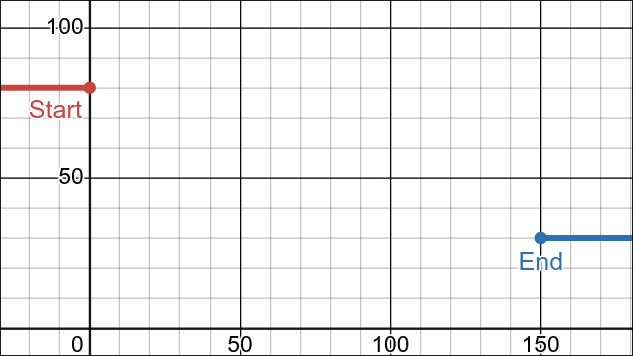
\includegraphics[width=15cm]{Start and End.png}

		\caption{The proposed start and end sections of the track}
		\end{center}


		\end{figure}

	\item The roller coaster could be faithfully modelled in 2D to simplify calculations as the width of the track and much of its geometry were not relevant in this case and we were not provided with specifications regarding the width available. 
	\item The task sheet defined the success criteria as causing the maximum amount of exhilaration, caused by "swift changes in direction, height and steepness". 
		
	\item It was required that the track be constructed of at least 3 or more types of functions, including at least two types that are covered in Unit 3 Topic 2. The functions covered were exponential, logarithms, and trigonometric functions, like sine, cosine, and tangent.
	\item It was decided that any calculations involving trigonometric functions would use radians, rather than degrees, in order for them to naturally oscillate more with smaller change in $x$.
	\item In order for the roller coaster to have sufficient speed to overcome any peaks or hills in the track, each successive peak should be at a lower height than any preceding it.

\end{itemize}
\end{itemize}


\subsection{Translation of aspects to Mathematical concepts and techniques}
\begin{itemize}
	\item Since the roller coaster had been assumed to be 2D, it's track could be represented on the Cartesian plane. This allowed us to use desmos to graph its track and perform calculations by letting 1 unit be 1 meter. 
	\item The derivative function of modelled section of track could be used to determine the gradient at that point and therefore be used to determine if the track exceeded the specified "Maximum Slope for safety" requirement provided by the task sheet. In this case, it was $-2$.
	\item "Swift changes in direction, height and steepness" could be translated to swift changes in the $y-$axis, and gradient. However, there was a maximum gradient specified that must be considered. 
	\item In order to achieve as much of a thrill as possible, the maximum slope should be reached whenever possible and appropriate.
	\item Cubic in general form


\end{itemize}


\section{Solve}
\subsection{Modelling in Desmos}
\subsubsection{The First Function}
\begin{itemize}
	\item Considering that the starting points for the middle section were already 80m in the air, it was determined that climbing further was futile as there was already sufficient height for the maximum gradient to be reached for a reasonable duration and the anticipation had already been built during the climb to the beginning of the middle section. 
	
	

	
	\item By defining the cubic generated as $f(x)$, desmos could generate the derivative function, $f'(x)$, automatically. Therefore by checking $f'(x)$ for intercepts with y=-2, it could be determined whether the generated cubic exceeded the maximum gradient.
	\item Clearly the first point will be $(80, 0)$ to connect with the start of the first segment. However we required for $f'(0)=0$ so the gradient so that the middle segment could smoothly connect to the first segment. By differentiating the general form of a cubic, it was found that $f'(x)=3ax^2+2bx+c$. The only part of the equation that did not have a coefficient of $x^n$ is $c$, therefore $c$ must be equal to $0$ for $f'(0)=0$.
	
	\item It was considered that during the first drop, a trigonometric function could be added so that more variability in the gradient could occur, therefore causing more of a thrill. 
	\item The sine function was chosen as it could be easily differentiated to the cosine function. 
	\item This meant that the second turning point of the cubic had to be placed so that it would coincide with one of the lower turning points of the sine function. 
	\item However the cubic was yet to be defined. We required maximum gradient during the drop. Since the derivative function was a quadratic, its lowest point could be considered the maximum gradient reached by the original.
	\item The $x$-coordinates of the turning points were found using the \textit{vertex} formula, which stated that for turning point $(x, y),\; x=\frac{-b}{2a}$.
	\item Considering the derivative function, $f'(x)=3ax^2+2bx$, by substituting the corresponding coefficients of $x^2$ and $x$ as $a$, and $b$ into the vertex formula respectively, it was found that the $x$-coordinates of the turning point were $\frac{-2b}{2\times3a}=\frac{-b}{3a}$.
	\item Therefore by finding $f'(\frac{-b}{3a})=-2$, a generic function could be found with minimum gradient -2, located at turning point. It was found that $f'(\frac{-b}{3a})=-2$ simplified to $b=\pm\sqrt{6a}$. Therefore the cubic $f(x)=ax^3\pm\sqrt{6a}x+d, a\geq0$ is found. 
	\item It was decided that the function inserted would be $f(x)=ax^3-\sqrt{6a}x+80, a\geq0$ as it placed the "drop" on the right hand side of the start of the coaster, and aligned the point on both tracks where their gradients were the same.
		\begin{figure}[h]
		\centering
		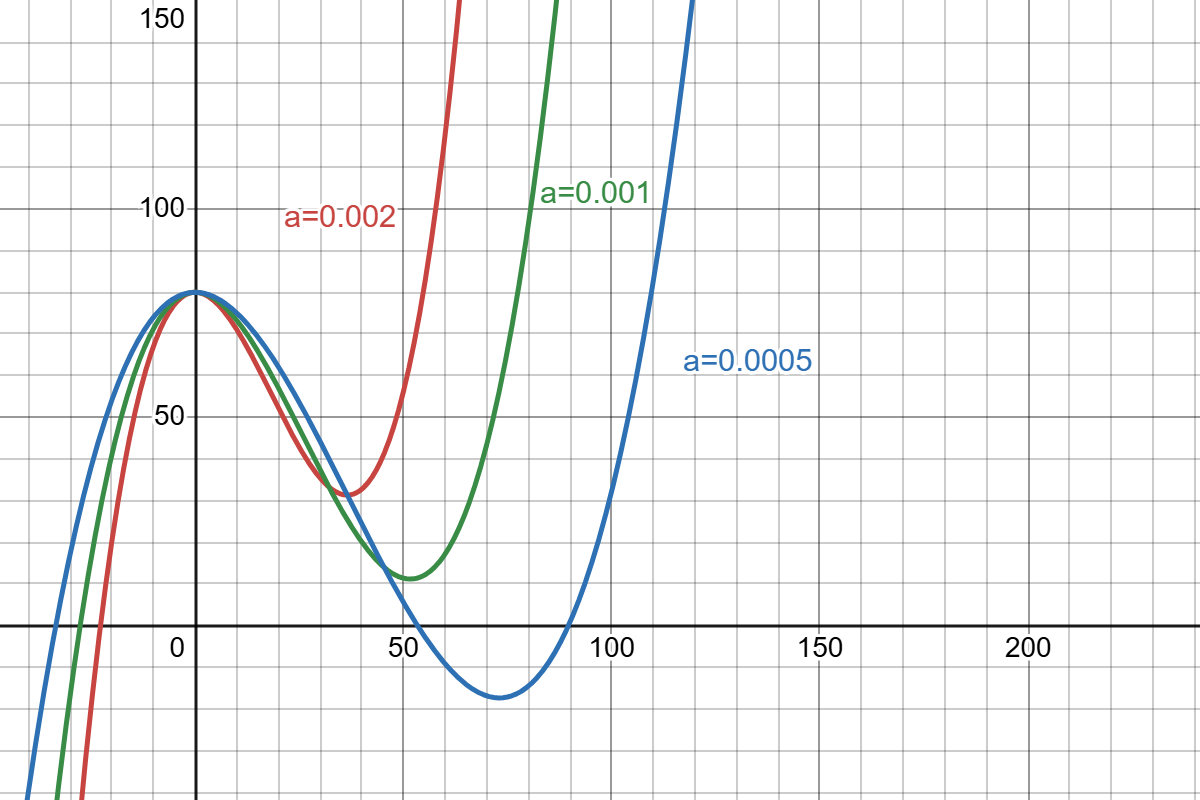
\includegraphics[width=15cm]{Eaxmple Cubic.png}
		\caption{Graphs of $f(x)=ax^{3}-\sqrt{6a}x^{2}+80$ with various $\mathbf{a}$ values}
	\end{figure}

	

	\item The end of the first function was chosen to be $f(30)$ as it was observed that letting it proceed further may have resulted in the end of the track being too low to the ground for a thrill to be achieved.
	\item It was required that the turning point be at $x=30$ so $f'(30)=0$ was considered. Solving for $a$ gave $a=\frac{2}{675}$
	\item Substituting this into $f(x)$ gave $f(x)=\frac{2}{675}x^{3}-\frac{2}{15}x^{2}+80$.
\end{itemize}
\subsubsection{The Second Function}
\begin{itemize}
	\item To connect the first and second functions, a point must be found where their gradients match.
	\item Consider $s(x)=a\sin(b(x+c))+d$. Therefore $s'(x)=ab\cos(b(x+c))$. Clearly the minimum gradient is defined by $ab\times-1$, where $a,b \epsilon \mathbf{N}$, as $a$ and $b$ both multiply with $\cos(b(x+c))$ which naturally oscillates between 1, and -1.
	\item However, if the function was allowed to continue for a period or more, the peak of the next oscillation would be smaller than the previous one. Therefore if the function was to continue, it must be modified in order for each successive peak to be lower. This was achieved though the creation of a new function, $c(x)=a\sin(b(x+c))+d+gx$, so that $c'(x)=ab\cos(b(x+c))+g$.
	\item Clearly now when $g<0$, the function will slope downwards throughout its oscillation. 

	\begin{figure}[h]
		\centering
		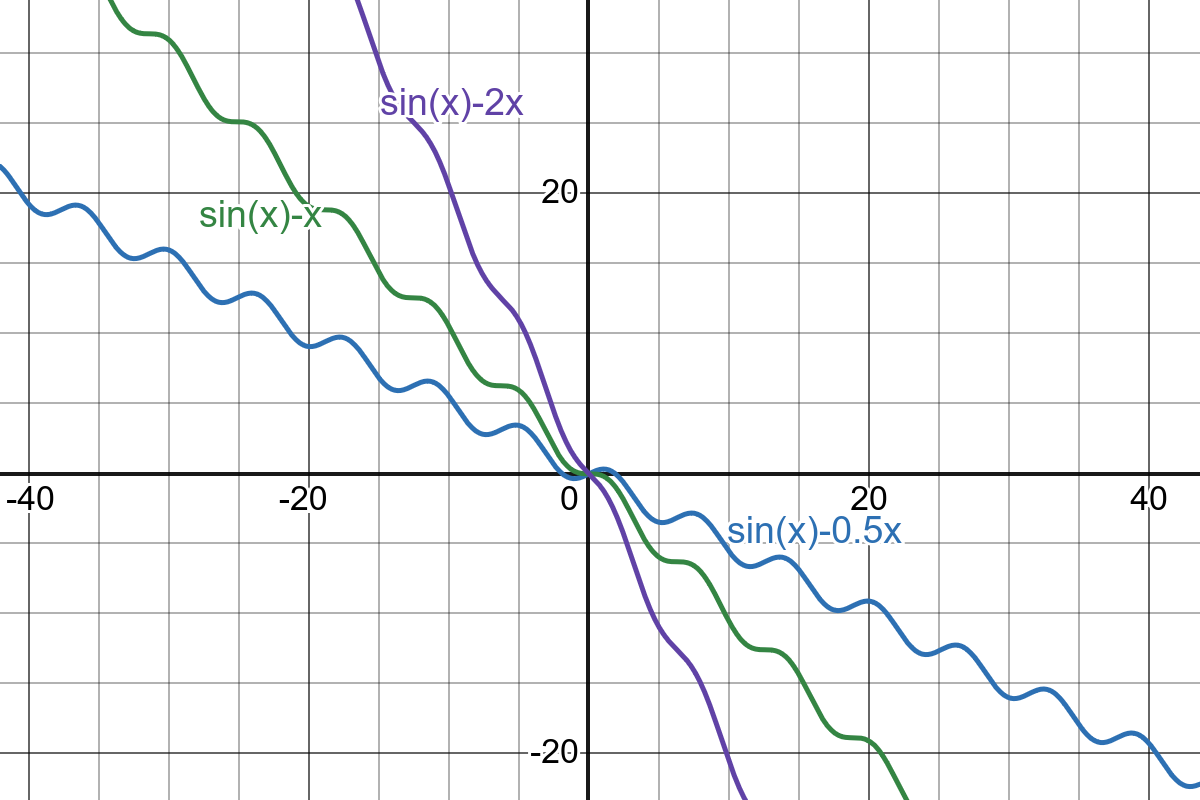
\includegraphics[width=15cm]{c(x).png}
		\caption{The function $y=sin(x)$ with various slopes applied}
	\end{figure}
	
	\item By letting $g=-0.1$, suitable values for $a$ and $b$ can be resolved. Clearly $ab\times-1-0.1=-2$ for minimum gradient to be achieved. Therefore through trial and error in Desmos it was found that for $c'(x)=-2$, $a=9.5,b=0.2$ were appropriate. Therefore all that was left to do was to let $f'(x)=c'(x)$, shifting horizontally until the minimums were at the same $x$ co-ordinates, then shift vertically shift using $d$ until the functions met.  
	\item It was found  that $9.5\times0.2\cos (0.2(30+c))-0.1=0 \Rightarrow c=-6.174775557$, and therefore $9.5sin(0.2(30-6.174775557))+d+3=40 \Rightarrow d=52.48683298$
\end{itemize}
\subsubsection{The Third Function}
\begin{itemize}
	\item It was decided that the third function would be an exponential that traveled downwards towards the ground, becoming more steep in the process. 
	\item Considering the general form of an exponential, $g(x)=ae^{b(x+c)}+d$, it was found that solving for variables $a, b, c$ and $d$ would require significant computation.
	\item Therefore it was decided that only $a$ and $b$ would need to be solved for, while $c=0$, and $d=0$.
	\item It was required that $g(80)=c(80)$, and $g'(80)=c'(80)$.
	\item Now that $g(x)=ae^{bx}$, $g'(x)=abe^{bx}$, we could solve for $a$ and $b$ using simultaneous equations.
	\item It was found that $a=\frac{c'(80)}{be^{80b}}$, therefore $g(80)=\frac{c'(80)}{be^{80b}}\times e^{80b}$. This gives $b=\frac{c'(80)}{c(80)}\approx -0.023308398873$.
	\item Since $a$ is a function of $b$, this also acts as a solution for $b$.
\end{itemize}






\section{Evaluate and Verify}



\end{document}